\documentclass[conference]{IEEEtran}
\IEEEoverridecommandlockouts
% The preceding line is only needed to identify funding in the first footnote. If that is unneeded, please comment it out.
%\usepackage{cite}
\usepackage{amsmath,amssymb,amsfonts}
\usepackage{algorithmic}
\usepackage{graphicx}
\usepackage{textcomp}
\usepackage{xcolor}

\usepackage{pdflscape}

\usepackage[utf8]{inputenc}
\usepackage{fancyhdr}
\usepackage{lastpage}

% Please add the following required packages to your document preamble:
\usepackage{multirow}
\usepackage[numbers]{natbib}

\usepackage{listings}
\usepackage{enumitem}
\usepackage{hyperref}
\usepackage{amsmath}

\hypersetup{
  citecolor=black,
  colorlinks=true,
  linkcolor=black,
  filecolor=magenta,      
	urlcolor=cyan
}

\usepackage{listings}
\usepackage{color}

\definecolor{dkgreen}{rgb}{0,0.6,0}
\definecolor{gray}{rgb}{0.5,0.5,0.5}

\definecolor{mauve}{rgb}{0.58,0,0.82}

\lstset{frame=single,
  language=C++,
  showstringspaces=false,
  columns=flexible,
  basicstyle={\small\ttfamily},
  numbers = none,
  numberstyle=\tiny\color{gray},
  keywordstyle=\color{blue},
  commentstyle=\color{dkgreen},
  stringstyle=\color{mauve},
  breaklines=true,
  breakatwhitespace=true,
  tabsize=2
}

\def\BibTeX{{\rm B\kern-.05em{\sc i\kern-.025em b}\kern-.08em
T\kern-.1667em\lower.7ex\hbox{E}\kern-.125emX}}

\fancypagestyle{fancylandscape}{
\fancyhf{} %Clears the header/footer
\fancyfoot{% Footer
\makebox[\textwidth][r]{% Right
  \rlap{\hspace{.75cm}% Push out of margin by \footskip
    \smash{% Remove vertical height
      \raisebox{4.87in}{% Raise vertically
        \rotatebox{90}{Page \thepage\ of \pageref{LastPage}}}}}}}% Rotate counter-clockwise
\renewcommand{\headrulewidth}{0pt}% No header rule
\renewcommand{\footrulewidth}{0pt}% No footer rule
}

\pagestyle{fancyplain}
\fancyhf{}
\fancyfoot[c]{Page \thepage\ of \pageref{LastPage}}
\renewcommand{\headrulewidth}{0pt}

\begin{document}

	\title{Socket Programming and Concurrency}

	\author{\IEEEauthorblockN{1\textsuperscript{st} Given Edward Patch}
	\IEEEauthorblockA{\textit{Software Engineer Student (of BSc Year 3)} \\
    \textit{Socket Programming and Concurrency}\\
    \textit{University of Wales Trinity St. Davids (of Tim Bashford)}\\
    Swansea, Wales \\
    Student ID: 1801492}}

     \maketitle
    
    \thispagestyle{plain}
    \pagestyle{plain}
    
    %\tableofcontents
	  %\vspace{.5cm}
    %\newpage
    \begin{abstract}
      Concepts of Socket Programming and Concurrency, including network protocols, models and synchronisation. An implementation of a networked rock, paper and scissors Android application, including the server.
    \end{abstract}

    \begin{IEEEkeywords}
        Socket Programming, Concurrency, Networking.
    \end{IEEEkeywords}

    \section{Introduction}
      This article illustrates interoperability within network protocols and the best way of implementing the method. Network protocols, including Transmission Control Protocol (TCP) and User Datagram Protocol (UDP), explain how they support the networking procedures and ensure data delivery. The synchronisation of the mentioned network protocols gives how I/O dispatch models perform. A problem of a three-way handshake, also known as `Two Generals' and the impacts of Maximum Transmission Unit (MTU) size on data transmission. The article also includes an implementation of a networked Rock, Paper and Scissors Android Application game that allows a max lobby of two users.

    \section{Network Protocols}
      A network protocol is a set of rules of how a network should handle how network packets (transmission of data) are transmitted and received between network nodes. Usually, the standard template of network protocols comes from an adaptation of the Open Systems Interconnection (OSI) model. Refer to section~\ref{sec:networkModel}, page~\pageref{sec:networkModel}. Designation of the TCP and UDP network protocols fit within the Internet of Things (IoT) category and provides a model that works well with the Internet standard. TCP relies on a connection type protocol, whereas UDP focuses on a connectionless protocol.

      After some observation from the Journal Article, `Experimental Performance Comparison between TCP vs UDP tunnel using OpenVPN' by Irfaan Coonjah~\cite{coonjah_experimental_2015}, the study carried out trials the performance between TCP and UDP using a Virtual Private Network (VPN) tunnel. The VPN platform the the author(s) chose was OpenVPN. Figure~\ref{fig:tcpudp-expset} displays a diagram of the experiment provided by the author~\cite{coonjah_experimental_2015}:-

      \begin{figure}[h]
        \centering
        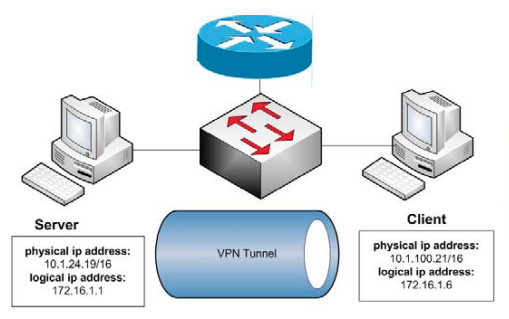
\includegraphics[width=\columnwidth]{Figures/TCPUDP-EXPSET.png}
        \caption{TCP vs UDP Tunnel Experiment Setup~\cite{coonjah_experimental_2015}}
        \label{fig:tcpudp-expset}
      \end{figure}

      Figure~\ref{fig:tcpudp-tcptun}: Graphs the TCP and UDP performance under a TCP VPN tunnel to observe the differential latency between the two protocols. The plots show that both protocols increase as the message size increases. TCP at zero megabytes (MB) sends data with a latency of zero seconds. The fact that TCP sends a message with a message size of zero is to add functionality to keep the connection between the two network nodes alive when there is no data to send during a period or to provide an initial warning that there is communication. Due to UDP being connectionless, there is no need for blank messages to send from node A to node B to keep the connection alive. UDP offers low latency compared to TCP up to the eight MB mark at thirty seconds of latency, whereas the TCP at eight MB takes thirty-five seconds of latency to transmit a message. However, at nine MB, the TCP performs faster than UDP by a marginal of one second, UDP being thirty-six seconds and TCP being thirty-seven seconds of latency. At ten MB, UDP performs faster than TCP by a margin of twelve, UDP performing at forty seconds of latency, whilst TCP performs at fifty-two seconds of latency.
      \begin{figure}[h]
        \centering
        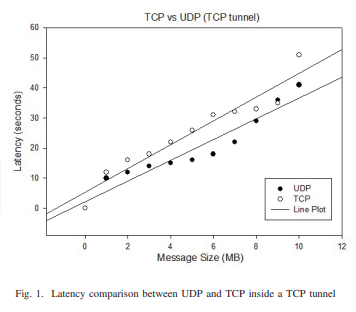
\includegraphics[width=0.70\columnwidth]{Figures/TCPUDP-TCPTUN.png}
        \caption{Latency of TCP/UDP through TCP Tunnel~\cite{coonjah_experimental_2015}}
        \label{fig:tcpudp-tcptun}
      \end{figure}

      Figure~\ref{fig:tcpudp-udptun}: Plots the performance of TCP and UDP performance under a UDP VPN tunnel to show the latency difference as the packet size changes. TCP and UDP start clustered from one to five MB packets ranging from five to fourteen seconds of latency. After this sequence, UDP strives with lower latency than TCP through the transition of five to ten MB, ranging from the latency of fifteen to twenty-five seconds for UDP and twenty-three to thirty-one seconds for TCP.
      \begin{figure}[h]
        \centering
        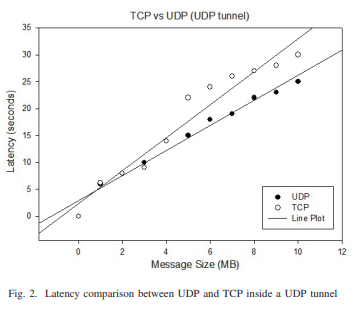
\includegraphics[width=0.70\columnwidth]{Figures/TCPUDP-UDPTUN.png}
        \caption{Latency of TCP/UDP through UDP Tunnel~\cite{coonjah_experimental_2015}}
        \label{fig:tcpudp-udptun}
      \end{figure}

      Comparing the two performances shows that UDP offers more significant message sizes within each data packet than TCP in TCP and UDP VPN tunnels. As TCP uses a prompt/transmit type of method to send data, the higher latency is reasonable if that data is acknowledged by the secondary node that data is awaiting, thus making sure the node prepares and handles the data before transmission happens. UDP protocol offers lower latency and benefit systems that do not need to wait for the data to be transmitted. However, by finding a sweet point of message size within the TCP network in whichever VPN tunnel, for example, one MB package size within the TCP tunnel. Due to the connection method within the TCP, an initial message to explain to Node B how the node should handle the receiving data. After the data is received, Node B can cross-reference the packet with a checksum initially sent to ensure the packet was sent and received correctly. This error handling enables the data to be transmitted correctly and increases the speed over time, keeping minimal latency.

      The idea of the `Generals Problem' is the thought process of setting up communications on a network that does not offer reliable stability. Referring back to splitting up packets and error-checking is essentially thought and designed using the three-handshake problem. TCP sends signals down multiple nodes within the network by synchronising transmitting, acknowledging and receiving, and acknowledging the final stage for the transmission. This method provides packet tracing to prevent any loss of information between each node. If the acknowledging signal is lost and never reaches Node A or Node B, this could cause an infinity loop problem as the nodes would be unable to communicate with each other if they received or not. Coming back to the `keep alive' empty message size helps prevent this from becoming a problem.

      MTU is a recommendation of the maximum data packet that a network can transmit and receive without any fragmentation of the network packets. The MTU size depends on the hardware and software within a network, and it is not always reliable when multiple maximum-sized packets over a TCP network could cause an increased latency time.

    \section{Network Models}
    \label{sec:networkModel}
      OSI, TCP/Internet Protocol (TCP/IP) and Information-Centric Networks (ICN) are three network model standards that offer different purposes for how the network handles the transmission of network packets. The OSI network model provides a layer abstraction that works in many network situations, making it a popular OSI model. OSI model contains seven layers, which are:-
      \begin{itemize}
        \item[] \textbf{Layer 7:} Application
        \item[] \textbf{Layer 6:} Presentation
        \item[] \textbf{Layer 5:} Session
        \item[] \textbf{Layer 4:} Transport
        \item[] \textbf{Layer 3:} Network
        \item[] \textbf{Layer 2:} Data Link
        \item[] \textbf{Layer 1:} Physical
      \end{itemize}

      The initial layer, Physical, focuses on identifying what devices are within the network to select the shortest path from the source node to the target node. The Physical layer is also responsible for sending unstructured data across the network. The second layer, Data Link, connects to each relevant node within the network to establish a connection. Within this layer, data from the Physical layer is processed into packets and tries to mend any errors that may exist from the Physical error. The Network layer found within the third position of the OSI model focuses on receiving packets from the previous layer. This layer is responsible for controlling where the nodes end up by the node addresses. The network layer positioned in the fourth position of the OSI model focuses on packet data error checking and delivery to guarantee that the target node within the server gathers the transmitted data with a higher success rate. The fifth layer, Session, helps create a session between clients and servers within the network. This layer focuses on communication, encryption, and decryption between the networked nodes. The presentation layer is the sixth layer that translates any data into a format that clients understand. This data goes to the Application layer, which indicates the front layer representing what the client may use, a service, application or other software interfaces. The data would reach an application at this point.

      The structure of the TCP/IP model is as follows:-
      \begin{itemize}
        \item[] \textbf{Layer 4:} Application
        \item[] \textbf{Layer 3:} Transport
        \item[] \textbf{Layer 2:} Internet Protocol
        \item[] \textbf{Layer 1:} Network Access
      \end{itemize}

      The Network Interface layer narrows the OSI model's Data Link and Physical layers into a single layer within the TCP/IP layer. The Internet Protocol layer is the Network layer of the OSI model, and the Transport layer is the same as the fourth layer of the OSI model. Application layer groups the Application, Presentation and Session layers within the OSI model.
      ICN uses three layers containing the following:-

      \begin{itemize}
        \item[] \textbf{Layer 3:} ICN Application
        \item[] \textbf{Layer 2:} ICN Forwarding
        \item[] \textbf{Layer 1:} Link
      \end{itemize}

      The ICN protocol offers a static (overlay or underlay) or a hybrid approach. The static approach of the ICN model is usually situated either in the overlay approach (above the Internet (second layer)) or the underlay approach (below the Internet (second layer)). Hybrid offers the network a way to manage data through two streams, either by the TCP/IP model or the ICN model, whereas the static method forces the ICN model within the TCP/IP model. 
      
      According to the Journal Article, `A Transport Layer and Socket API for (h)ICN: Design, Implementation and Performance Analysis' by Mauro Sardara~\cite{sardara_transport_2018} states `Each layer has different objectives and constraints. Each layer manages resources of different capacities implying trade offs while multiplexing/demultiplexing name data from one layer to another.' The statement by Mauro Sardara~\cite{sardara_transport_2018} suggests that the ICN layers are responsible for compressing data and sending it to the next layer, when the ICN model completes the end transfer decompresses the data making it heavier again. However, by observing the static and hybrid approaches of the ICN model, a ICN static approach could seem useless for performance reasons. The static ICN provides security to the TCP/IP layers, backed up by Mauro Sardara~\cite{sardara_transport_2018}, `...network-layer counterparts provides several benefits in term of packet processing and security'. A hybrid approach could increase performance and provide a unpredictable security approach as the network could choose to accept the TCP/IP or ICN model to process the data transmission.

      TCP/IP model with visualisation of ICN overlay and underlay approaches. The ICN layer exists above the Internet Protocol layer if the ICN overlay is present. Otherwise, the ICN layer belongs below the Internet Protocol layer.
      \begin{itemize}
        \item[] \textbf{Layer 4:} Application
        \item[] \textbf{Layer 3:} Transport
        \item[] \textbf{Overlay Layer:} ICN (overlay approach)
        \item[] \textbf{Layer 2:} Internet Protocol
        \item[] \textbf{Underlay Layer:} ICN (underlay approach)
        \item[] \textbf{Layer 1:} Network Access
      \end{itemize}

    \section{Network Syncronisation}
      The network synchronisation deals with the time and frequency of message transmissions. The software runs with a series of instructions, and when another node transmits information to a device, the software within the network would have to decide to stop and wait or continue running the network. If a node waits for too long and has no idea whether the data is transmitted or not, then the network could wait forever, resulting in a network crash. The most popular network synchronisation is Network Time Protocol (NTP). NTP is based on a UDP model to communicate within the network structure. A few network synchronisation techniques that exist are as follows:-
      \begin{itemize}
        \item Plesiochronous (Asynchronous)-
        Plesiochronous network synchronisation does not rely on a clock for transmission to commence. This type of communication means that messages are not sent constantly to keep communication alive within a network and can transmit or receive without calculating the time and frequency of the transmission. This type of network synchronisation helps with unpredictable communication that has no time frame for the transmission's completion and enables a node to continue with the current process whilst the other node is processing the given job within the network.
        
        \item Synchronous -
        This technique relies on a NTP to synchronise data communication. As the synchronous technique relies on time to transmit data, a reliable clock source like Global Navigation Satellite System (GNSS), Coordinated Universal Time (UTC) or Global Positioning System (GPS) helps ensure that the network remains in sync.
      \end{itemize}
    \section{Implementation}
      An implementation of a Rock, Paper and Scissors application with Java and Java Native Interface (JNI) coding and a server written in C++ with Linux libraries for both Client and Server sides. The implementation uses four states, search game, find player, play game and end game. The server only supports two plays and controls three main activities within the Java Android application the start screen, find a game and play the game. The start game is the activity where the user can enter the username. Find a game is an activity where the user connects with another available player. Playing the game is the activity where the two users select Rock, Paper or Scissors before three seconds run out; the players have three turns before the game ends.

      Figure~\ref{fig:startActivity}: The start activity is the first instance that loads for the client. This figure shows a welcome screen with an animated logo, using Java threads and timers and a username input.
      \begin{figure}[h]
        \centering
        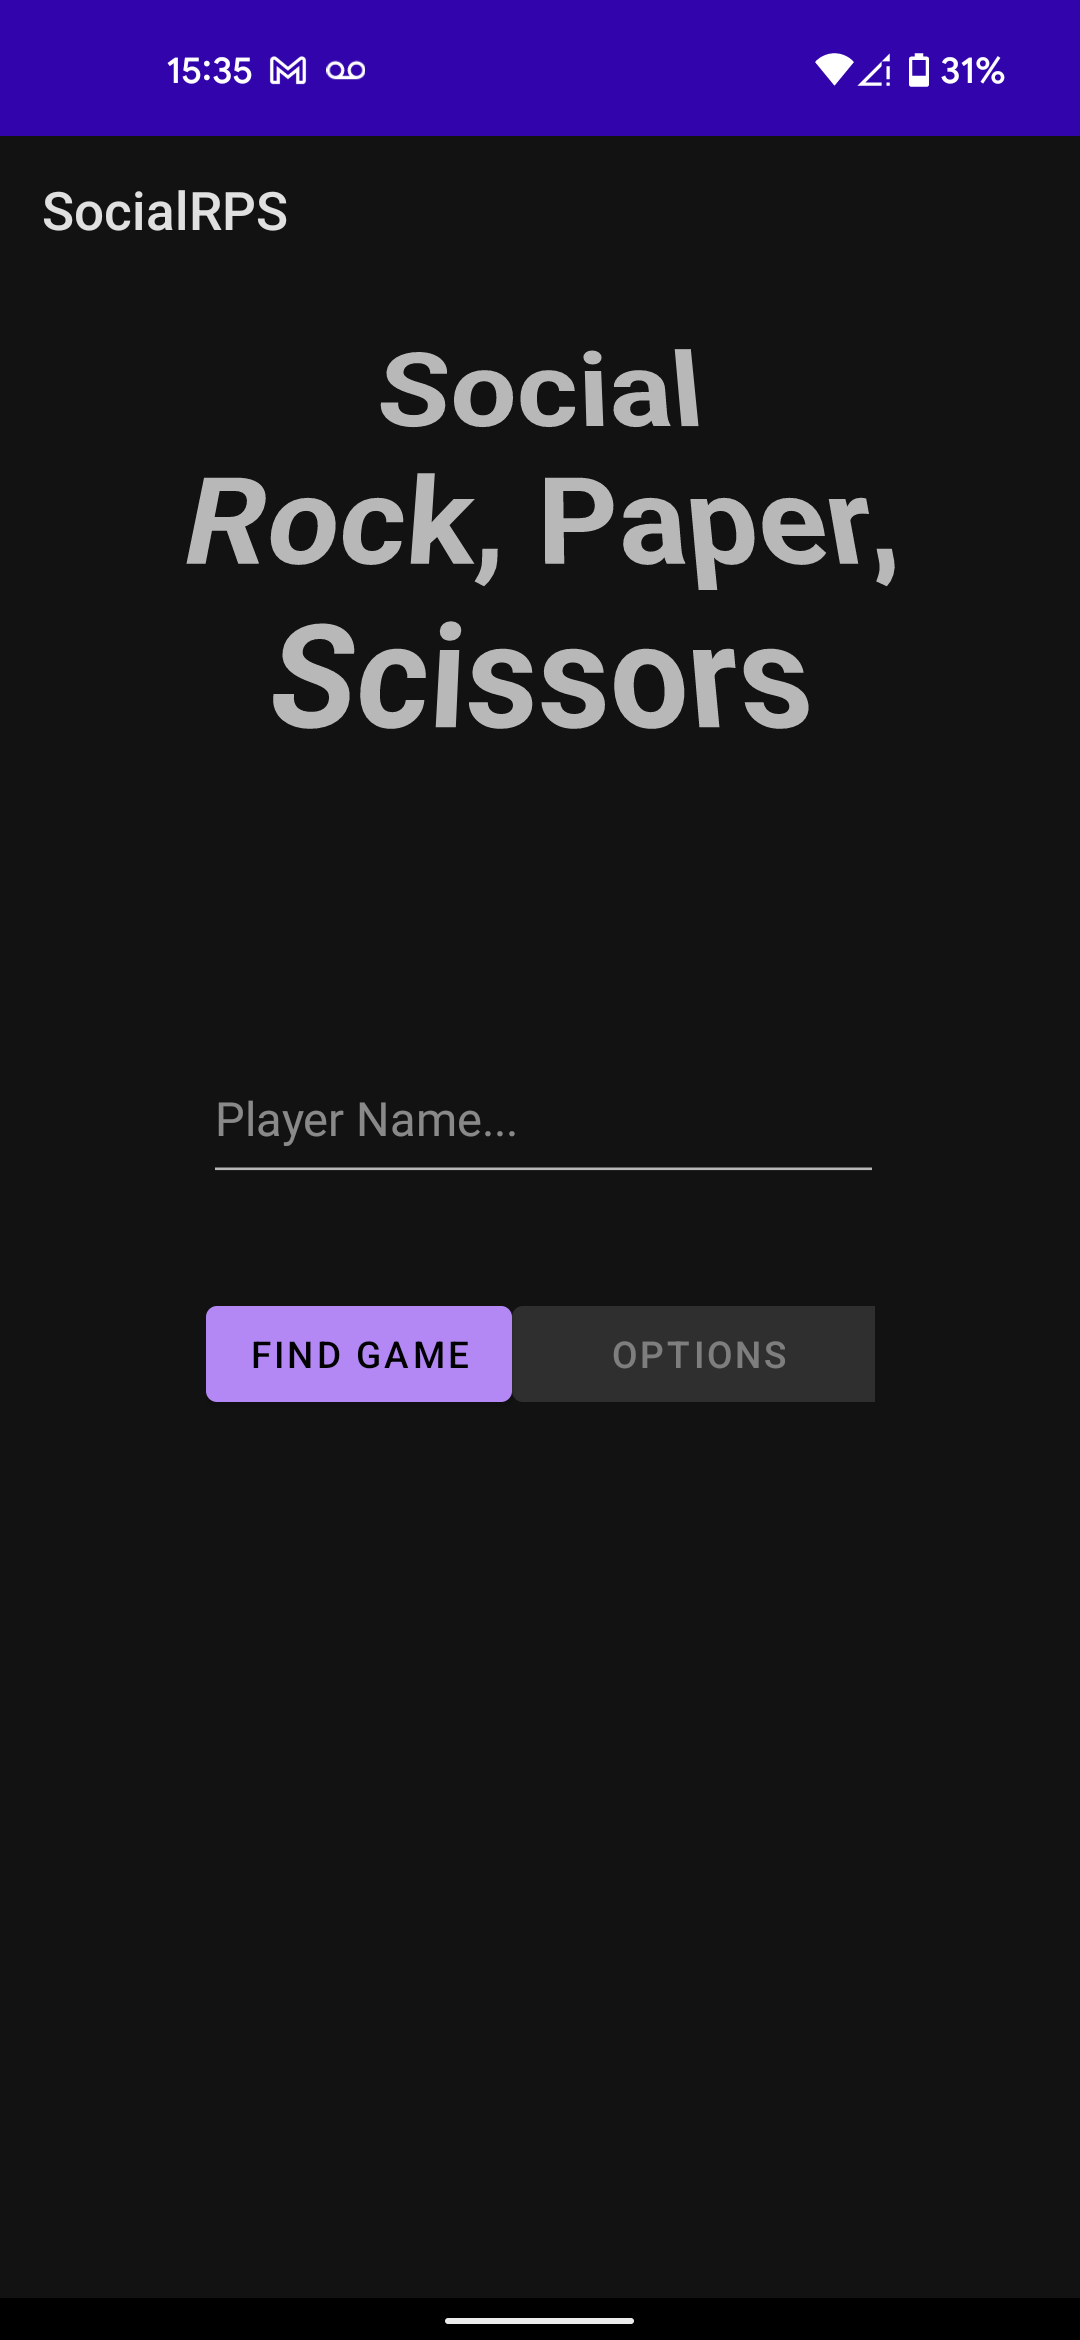
\includegraphics[width=0.22\columnwidth]{Figures/StartActivity.png}
        \caption{Start Activity - The start screen of the application}
        \label{fig:startActivity}
      \end{figure}

      Figure~\ref{fig:startActivityAnim}: The figure shows some motion of the animated logo.
      \begin{figure}[h]
        \centering
        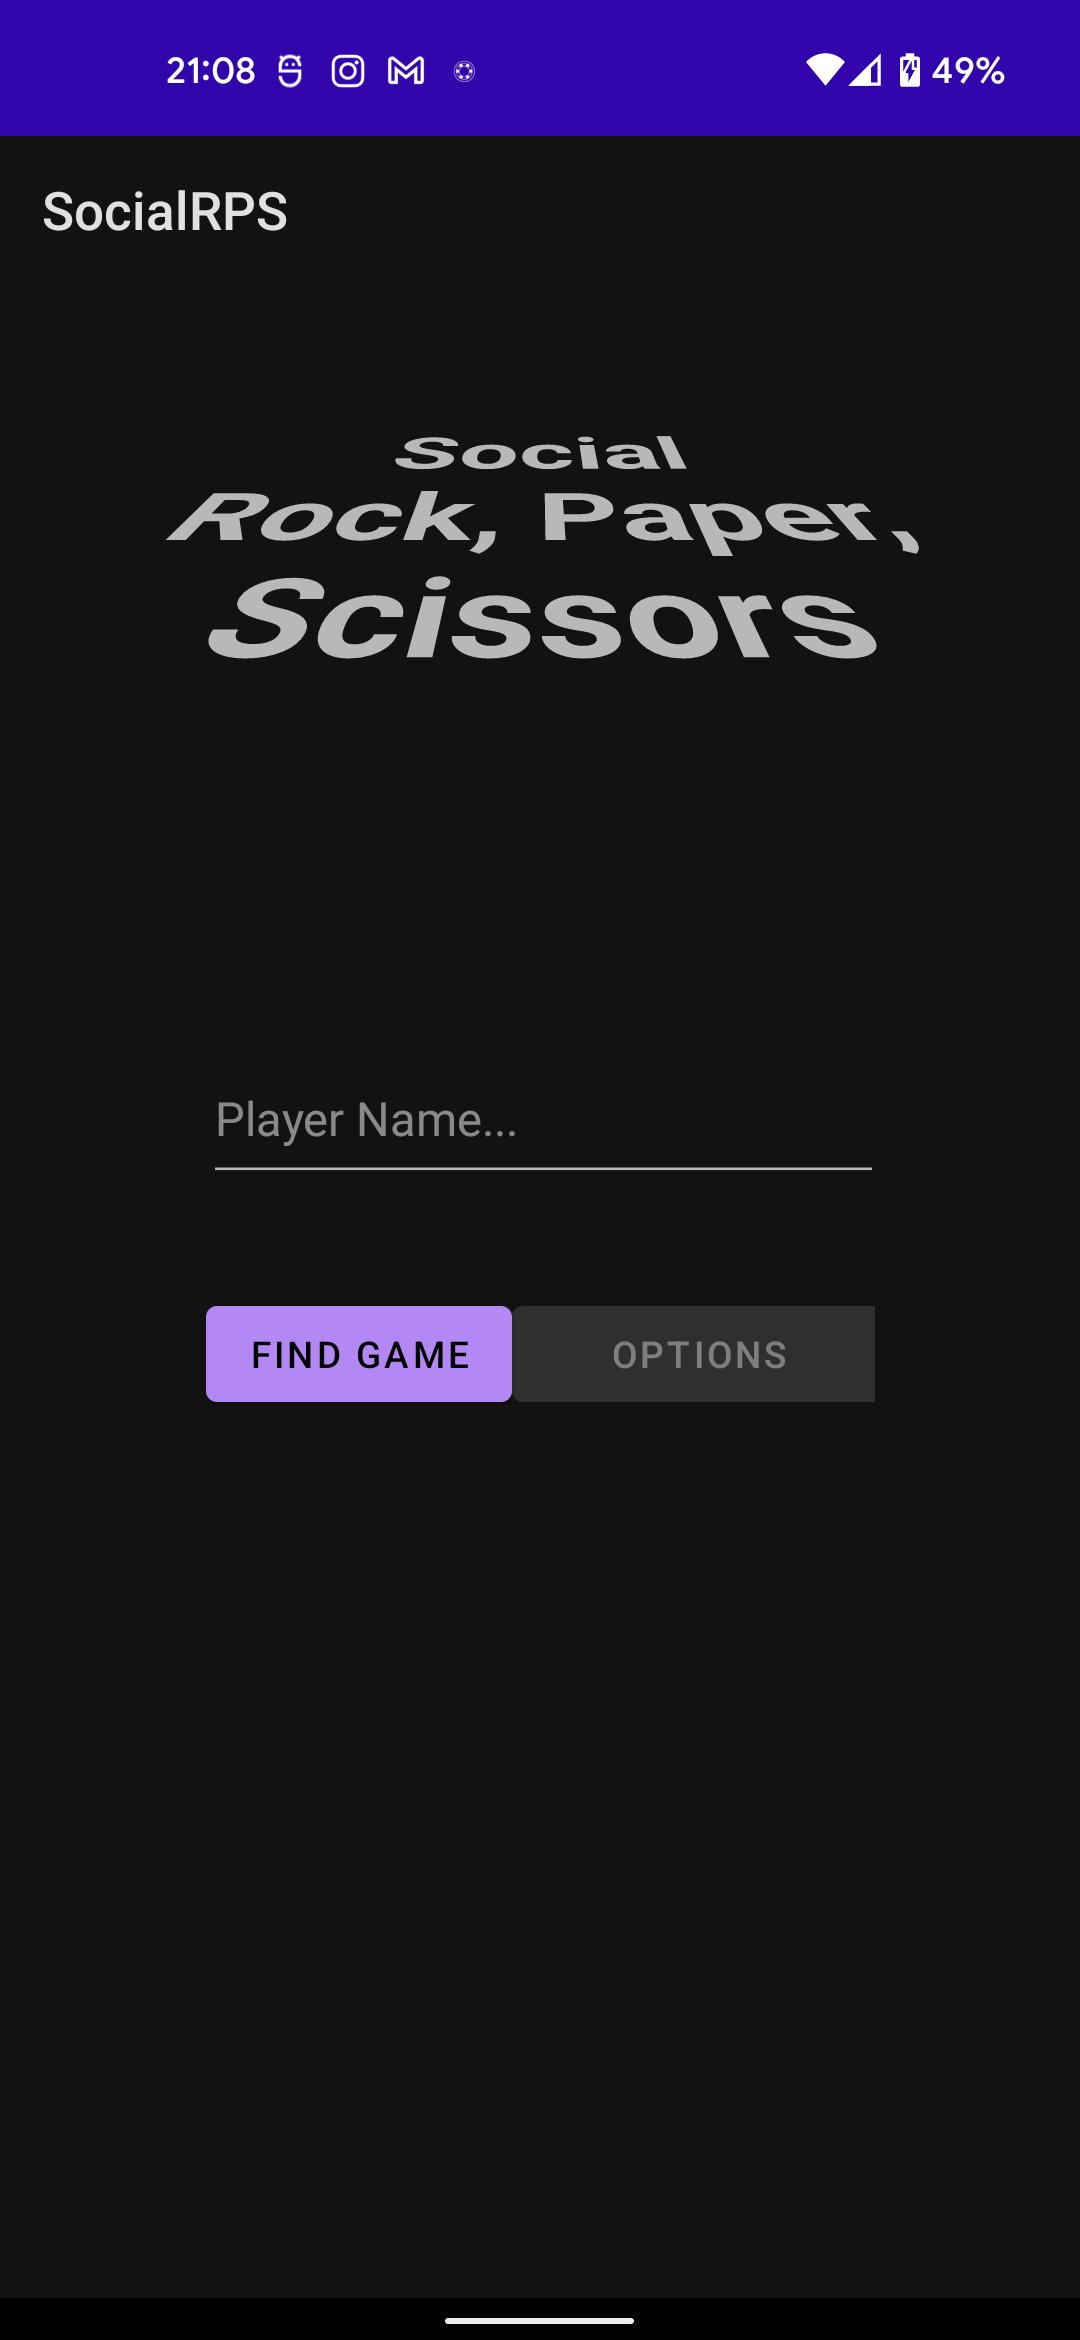
\includegraphics[width=0.27\columnwidth]{Figures/StartActivityHalfYRotation.png}
        \caption{Start Activity - Logo Rotation - Y-axis}
        \label{fig:startActivityAnim}
      \end{figure}

      Figure~\ref{fig:enterPlayerName}: After the user tries to start finding a game without entering a username, the application will display an error message reading `Please enter a player name!'.
      \begin{figure}[h]
        \centering
        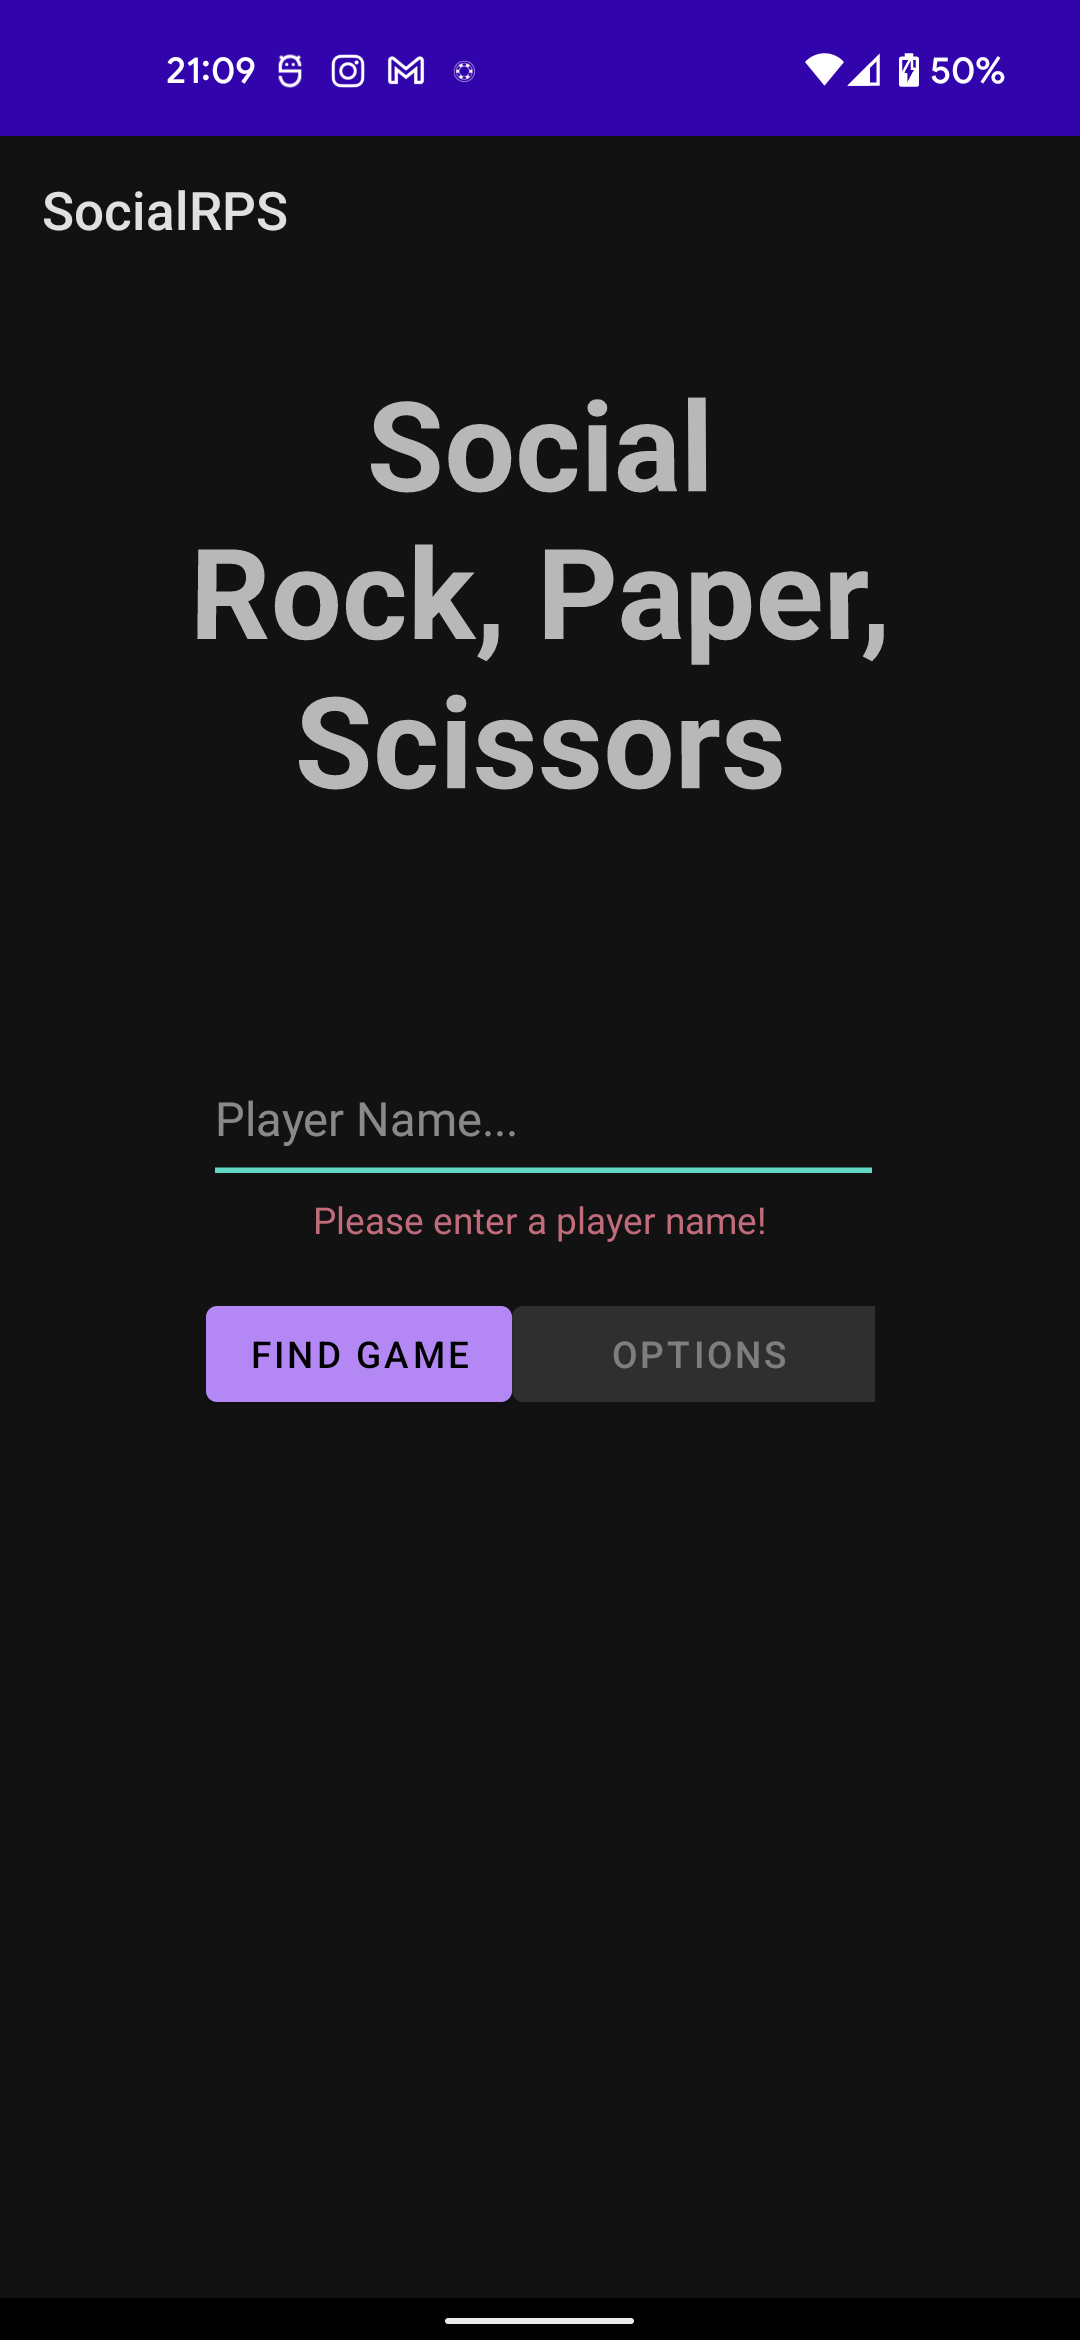
\includegraphics[width=0.27\columnwidth]{Figures/EnterPlayerName.png}
        \caption{Start Game Activity - Enter Player Name}
        \label{fig:enterPlayerName}
      \end{figure}

      Figure~\ref{fig:spaceCharacters}: Illustration of the space character error if a player attempts to find a game with a space within the username input.
      \begin{figure}[h]
        \centering
        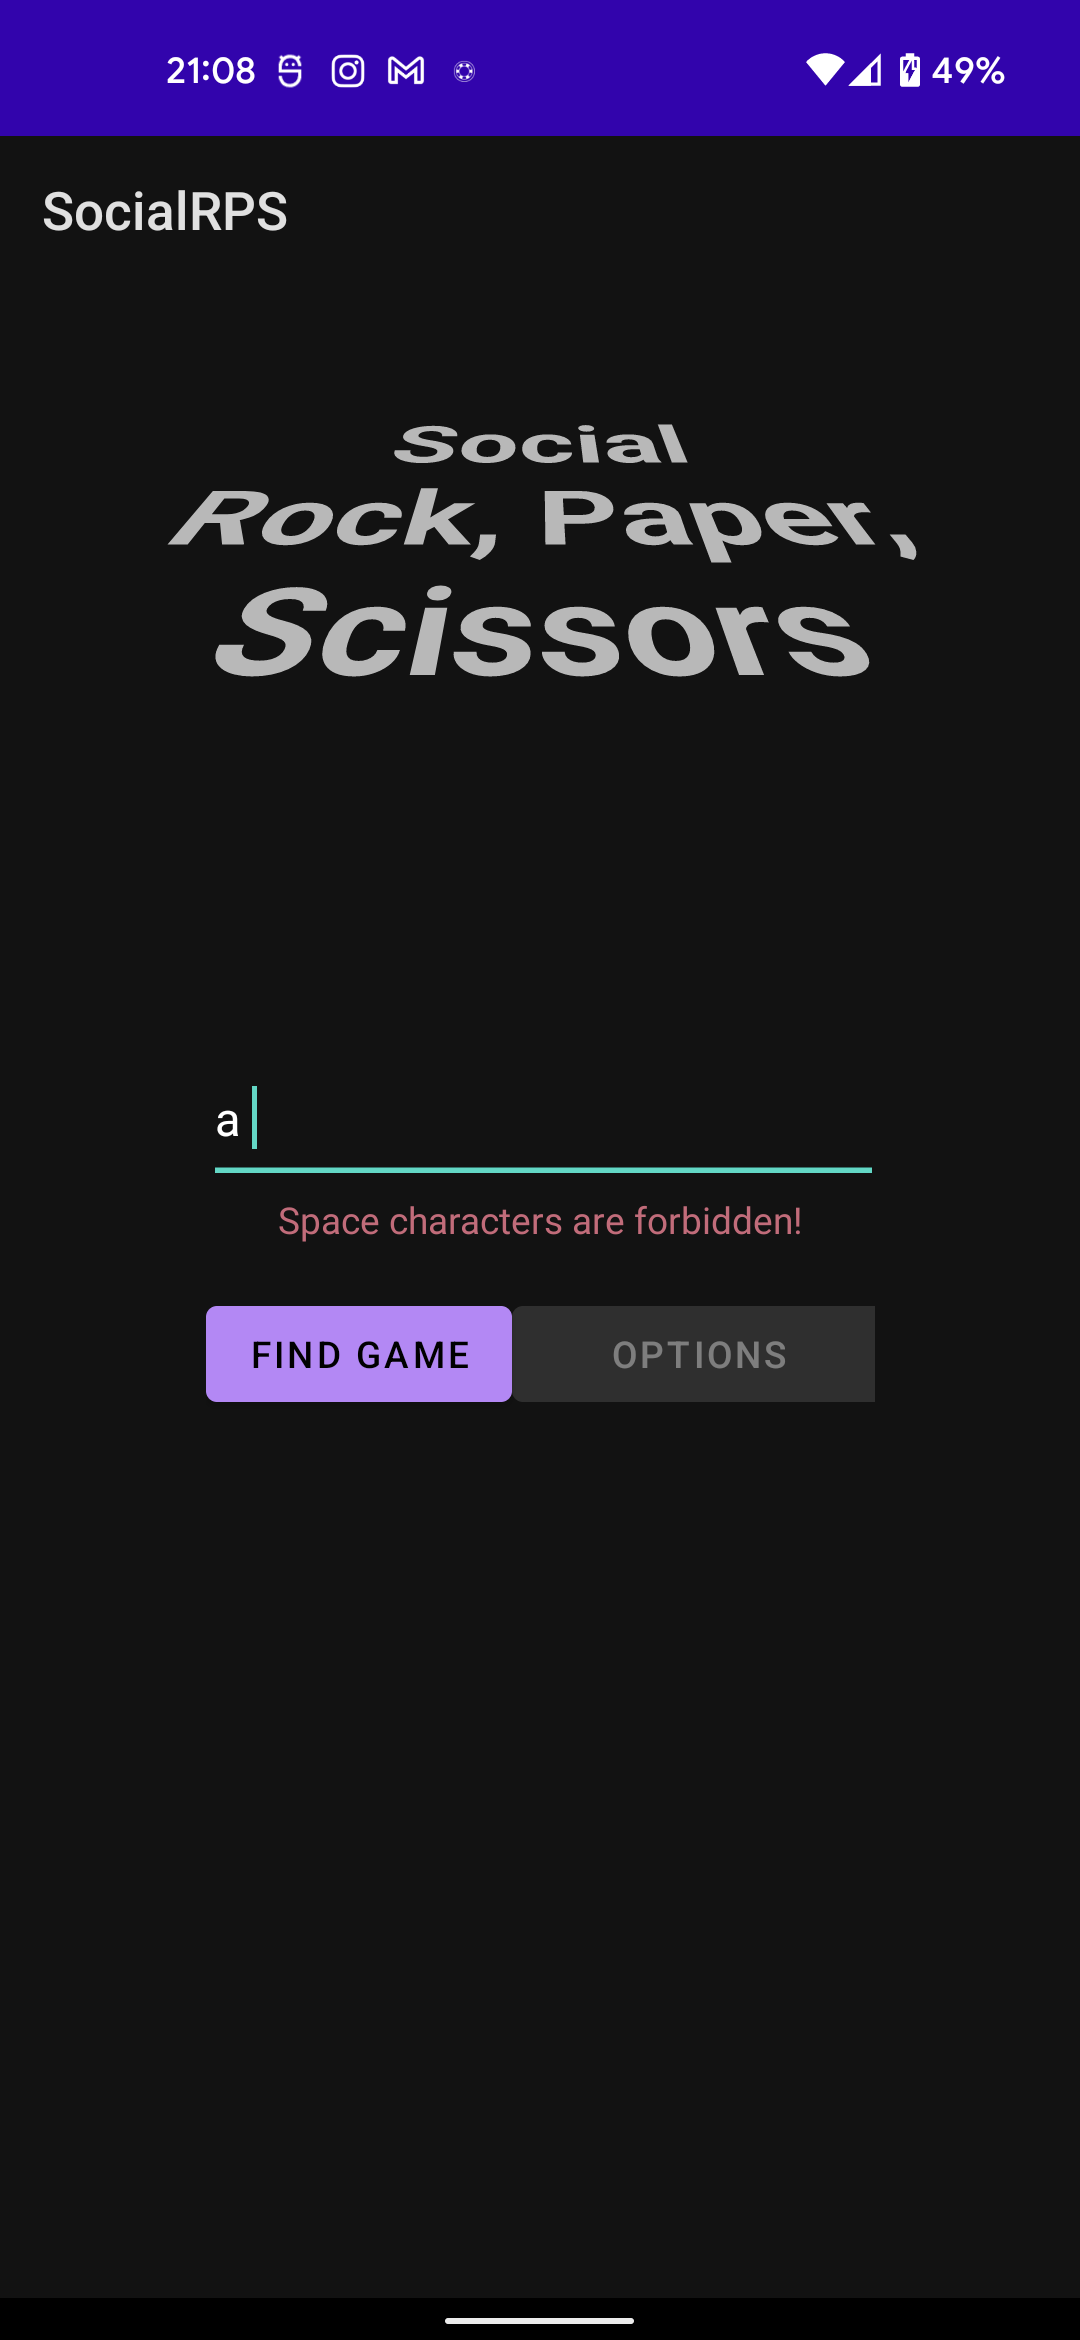
\includegraphics[width=0.27\columnwidth]{Figures/SpaceCharacters.png}
        \caption{Start Game Activity - Space Character Error}
        \label{fig:spaceCharacters}
      \end{figure}

      Figure~\ref{fig:findGame}: Displays the find game activity, which shows an animation using a Java thread and timer to inform the client that the application is trying to establish a connection with another player.
      \begin{figure}[h]
        \centering
        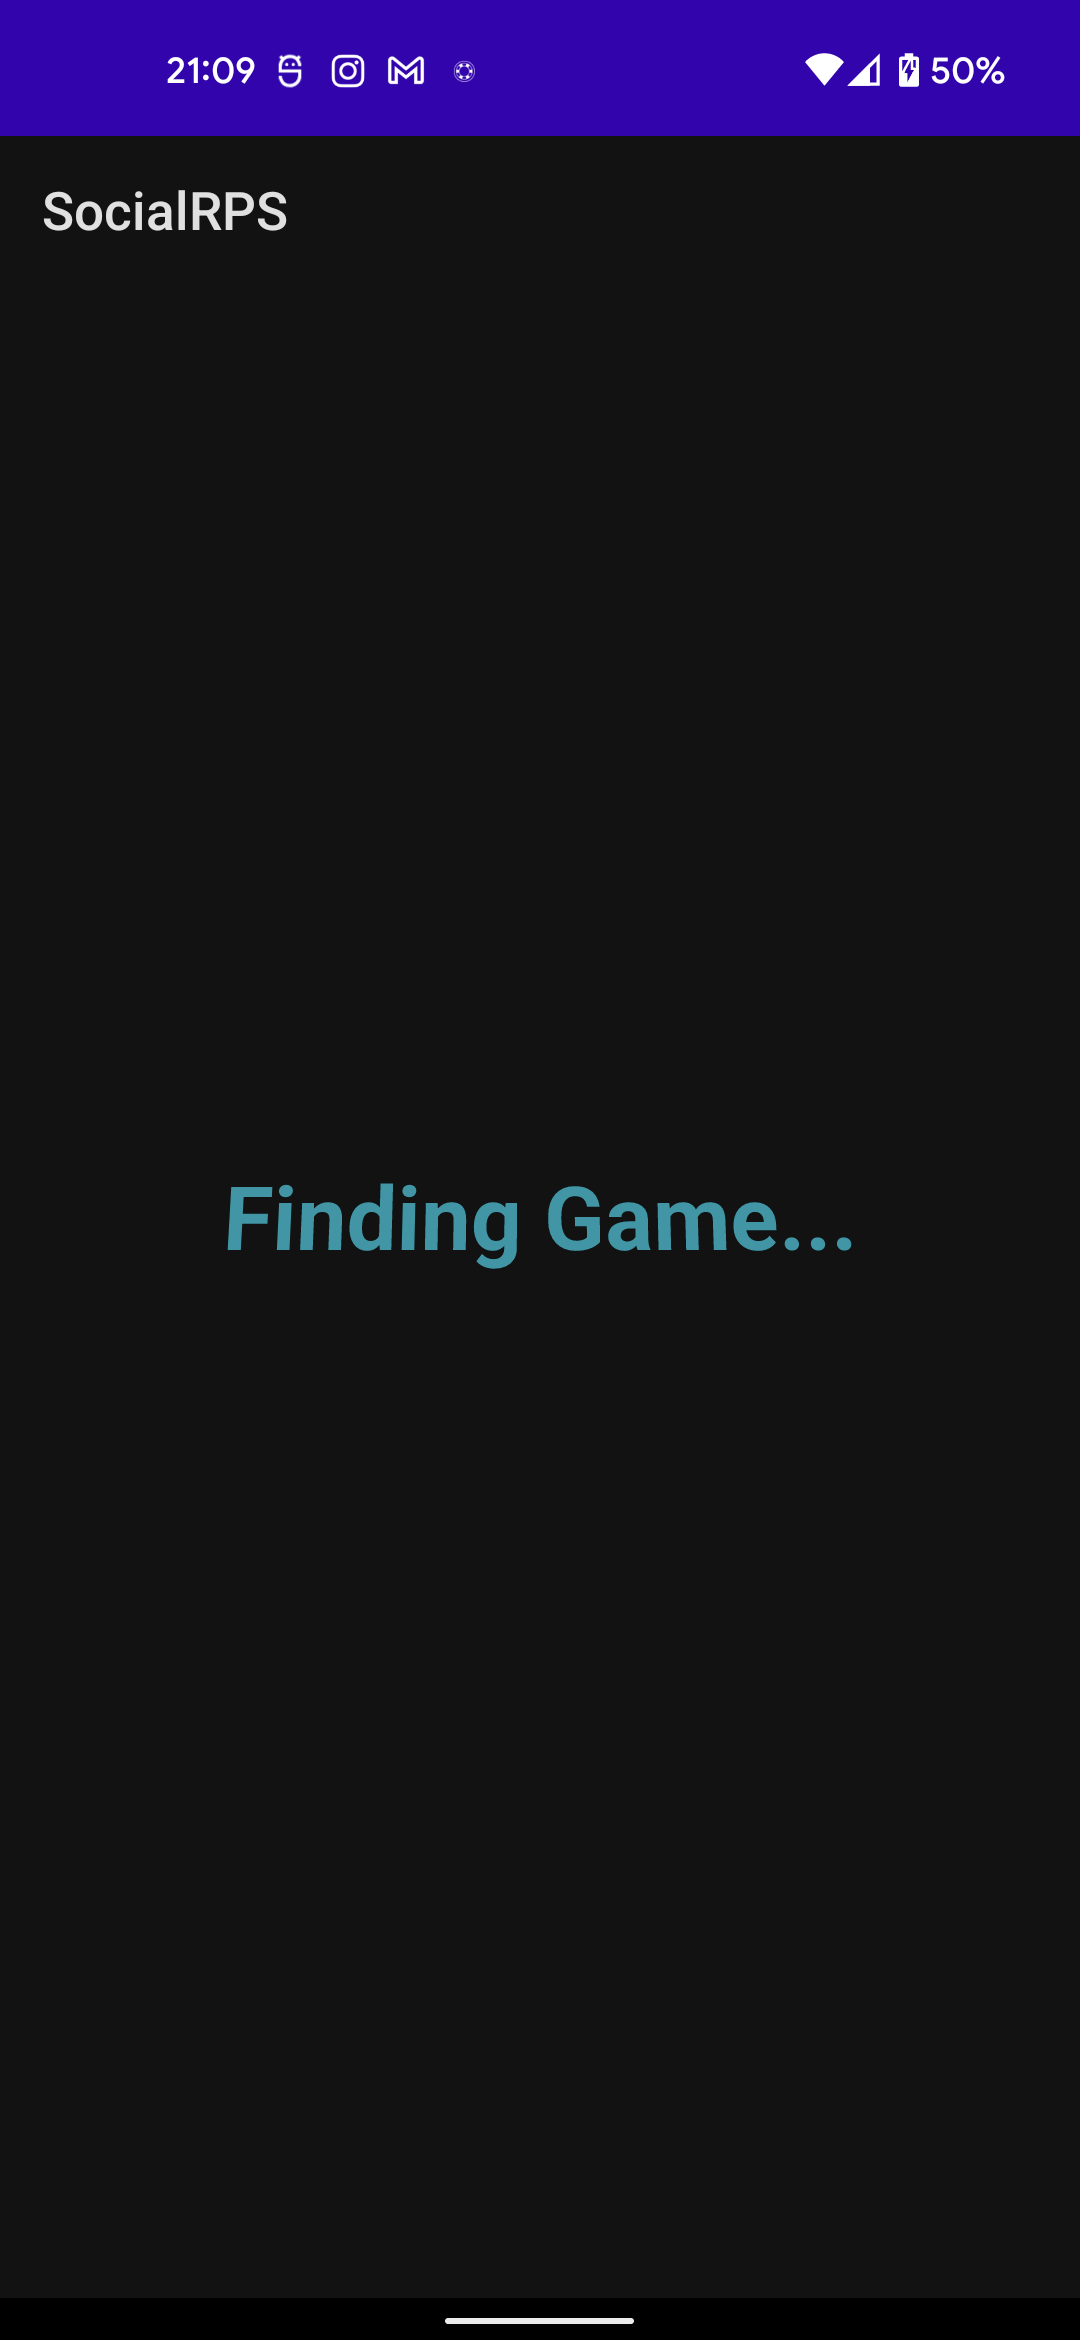
\includegraphics[width=0.25\columnwidth]{Figures/FindingGame.png}
        \caption{Find Game Activity - Finding Game}
        \label{fig:findGame}
      \end{figure}

      Figure~\ref{fig:findGameAnim}: The figure shows some motion of the animated logo.
      \begin{figure}[h]
        \centering
        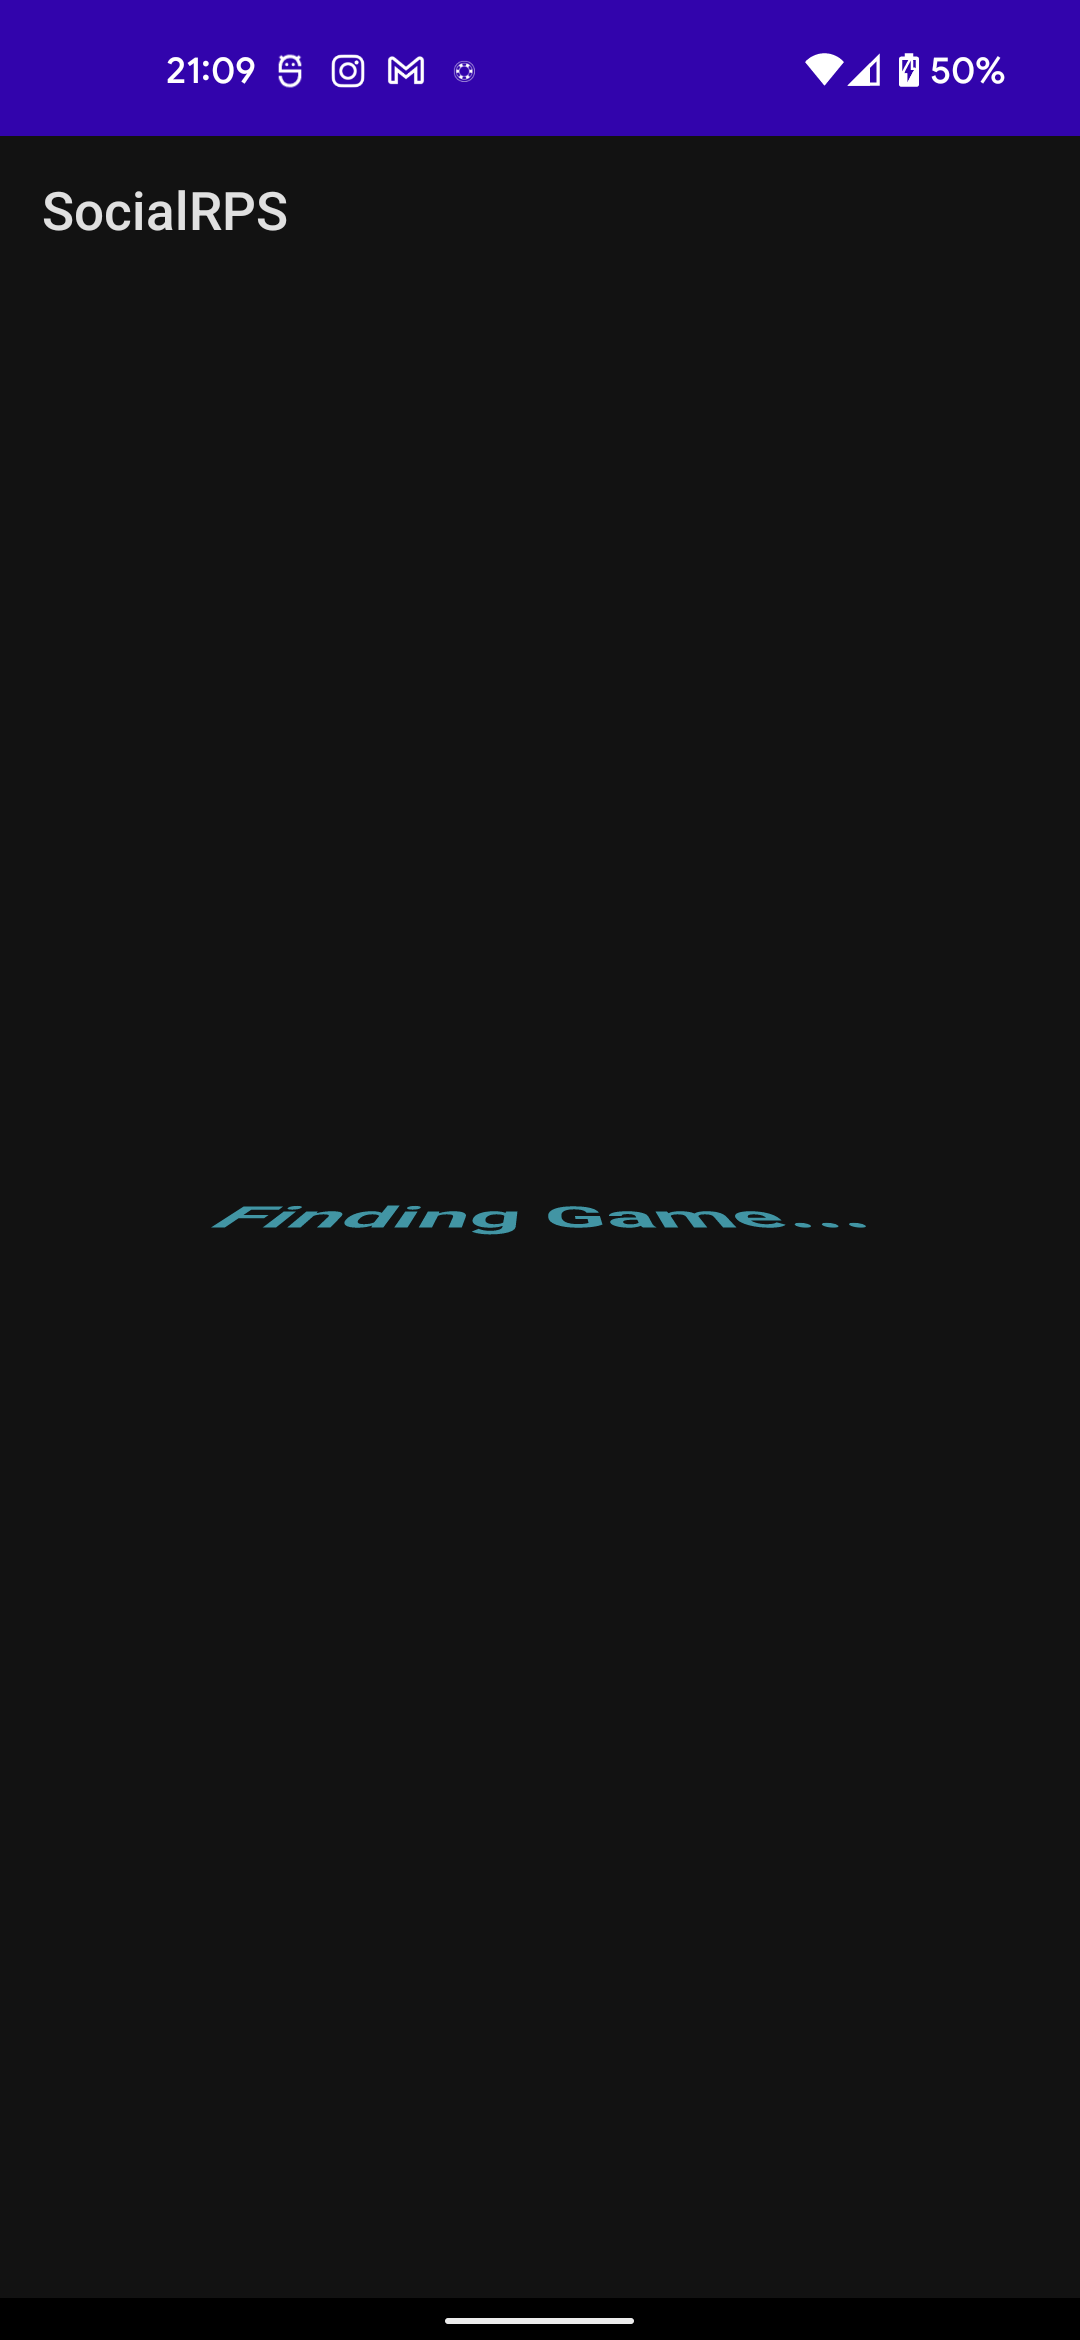
\includegraphics[width=0.25\columnwidth]{Figures/FindingGameYRotation.png}
        \caption{Find Game Activity - Logo Rotation - Y-axis}
        \label{fig:findGameAnim}
      \end{figure}

      Figure~\ref{fig:actions}: Within the Play Game activity, the user has an option to communicate and play a game of Rock, Paper or Scissors with the second player. The timer indicates the time the user has to make a selection. Otherwise, the turn is voided and counts as a loss.
      \begin{figure}[h]
        \centering
        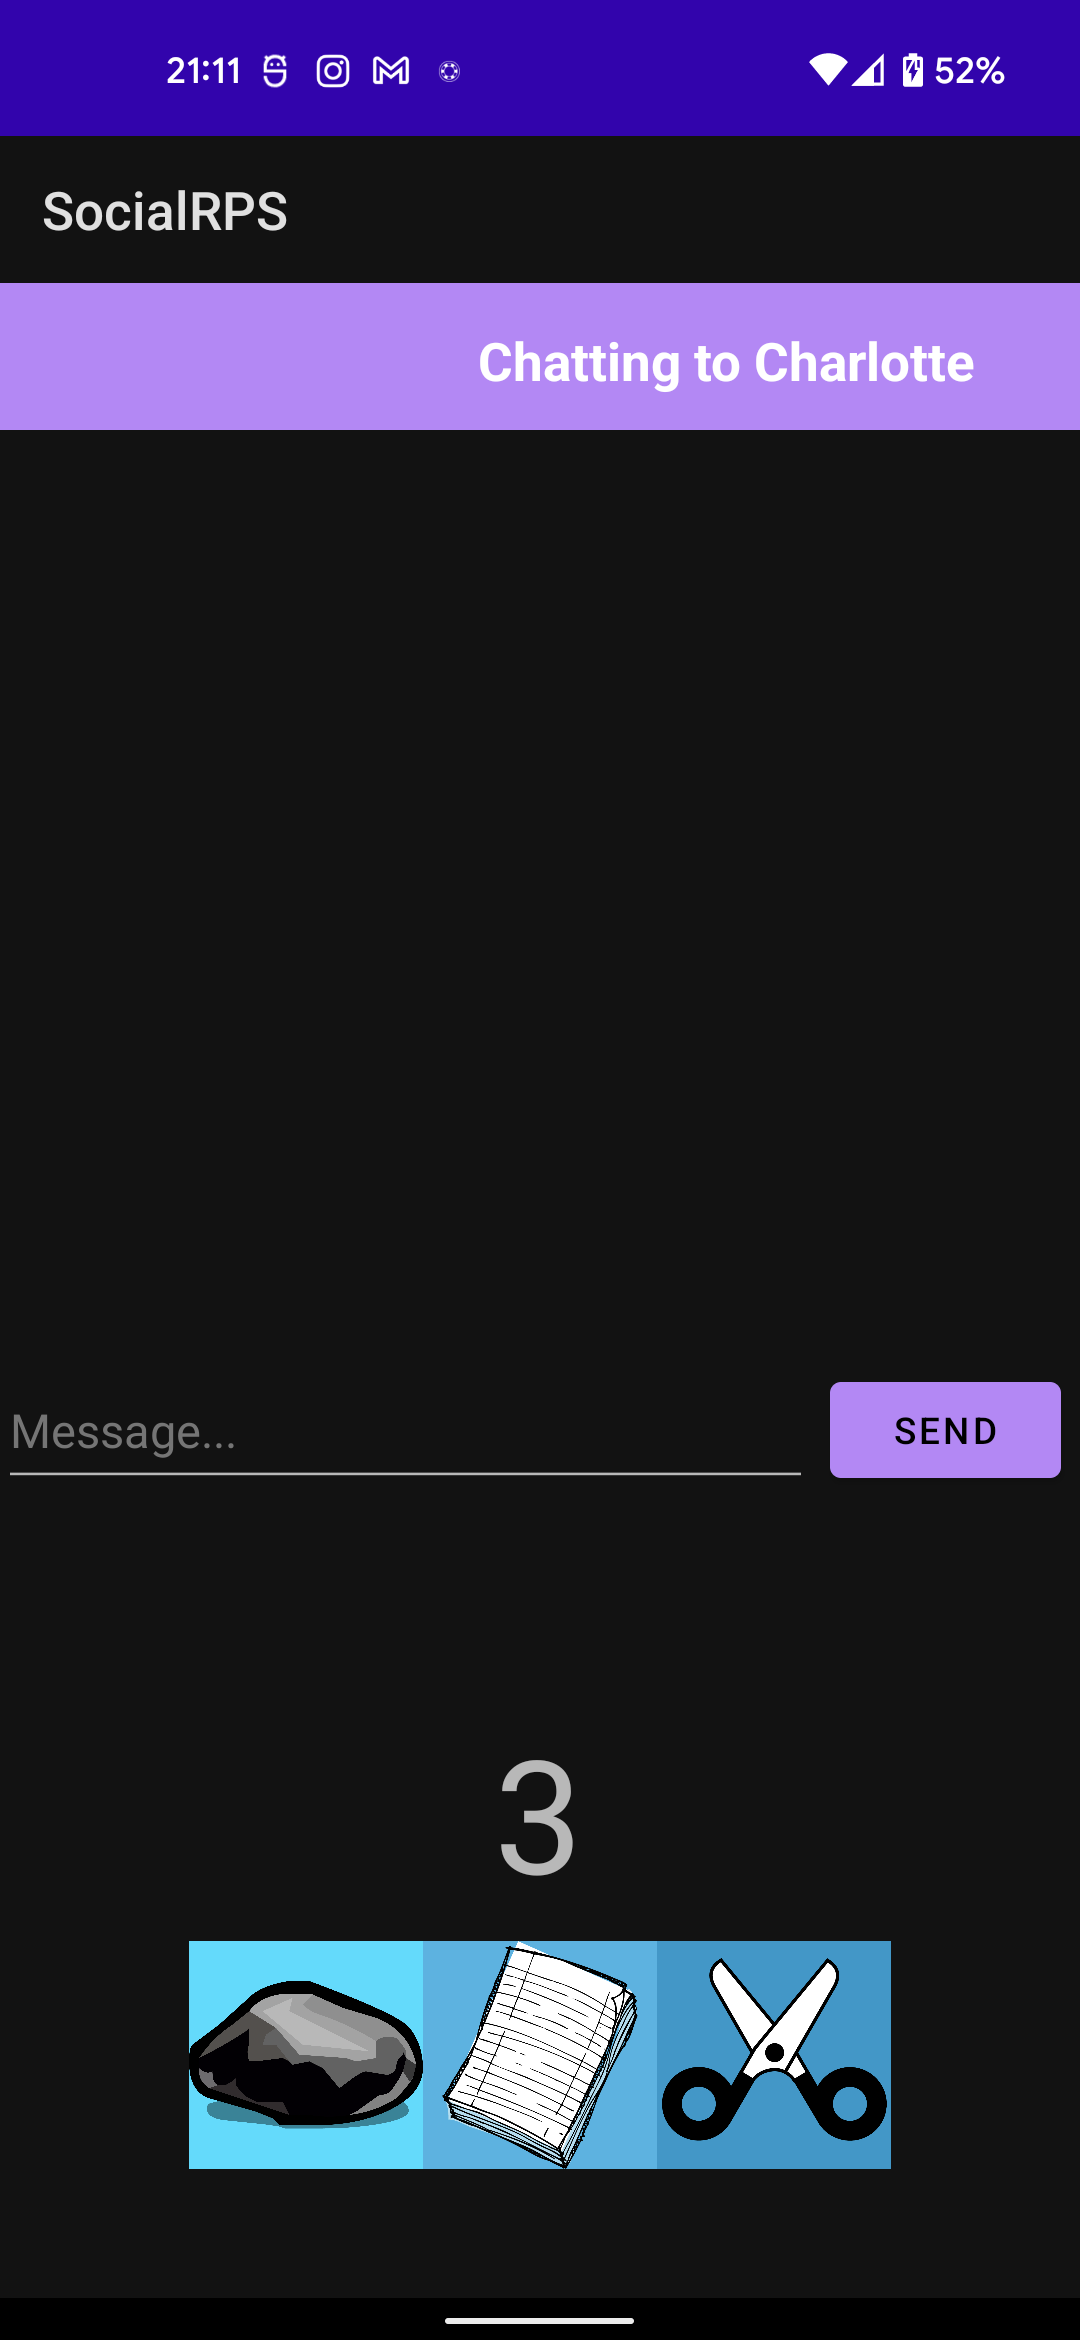
\includegraphics[width=0.25\columnwidth]{Figures/Actions.png}
        \caption{Play Game Activity - Actions}
        \label{fig:actions}
      \end{figure}

      Figure~\ref{fig:actionsRock}: The figure shows what the client sees if the user touches the Rock action button.
      \begin{figure}[h]
        \centering
        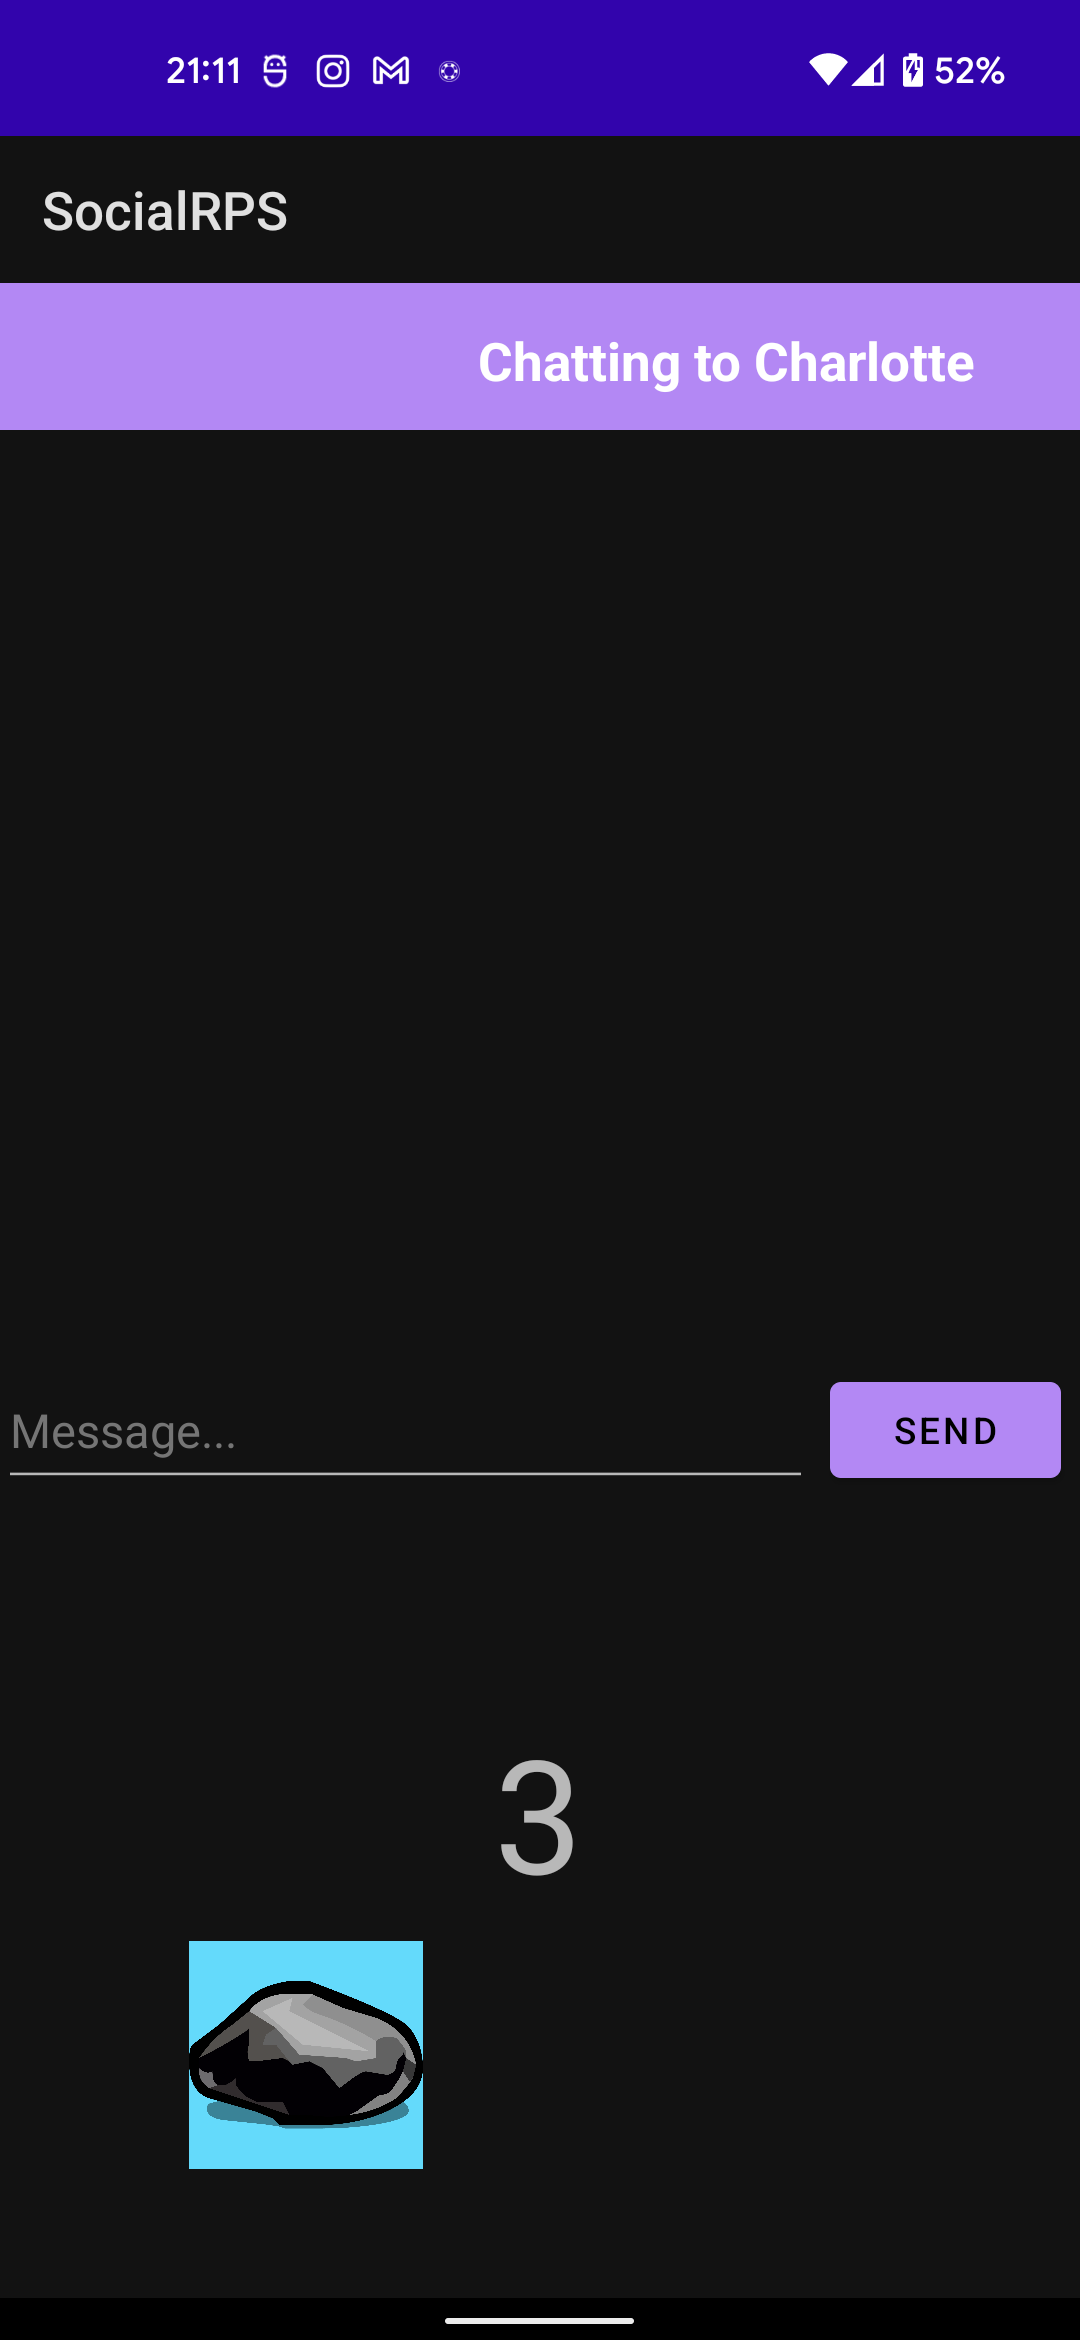
\includegraphics[width=0.27\columnwidth]{Figures/RockAction.png}
        \caption{Play Game Activity - Rock Action}
        \label{fig:actionsRock}
      \end{figure}

      Figure~\ref{fig:actionsPaper}: The figure shows what the client sees if the user touches the Paper action button.
      \begin{figure}[h]
        \centering
        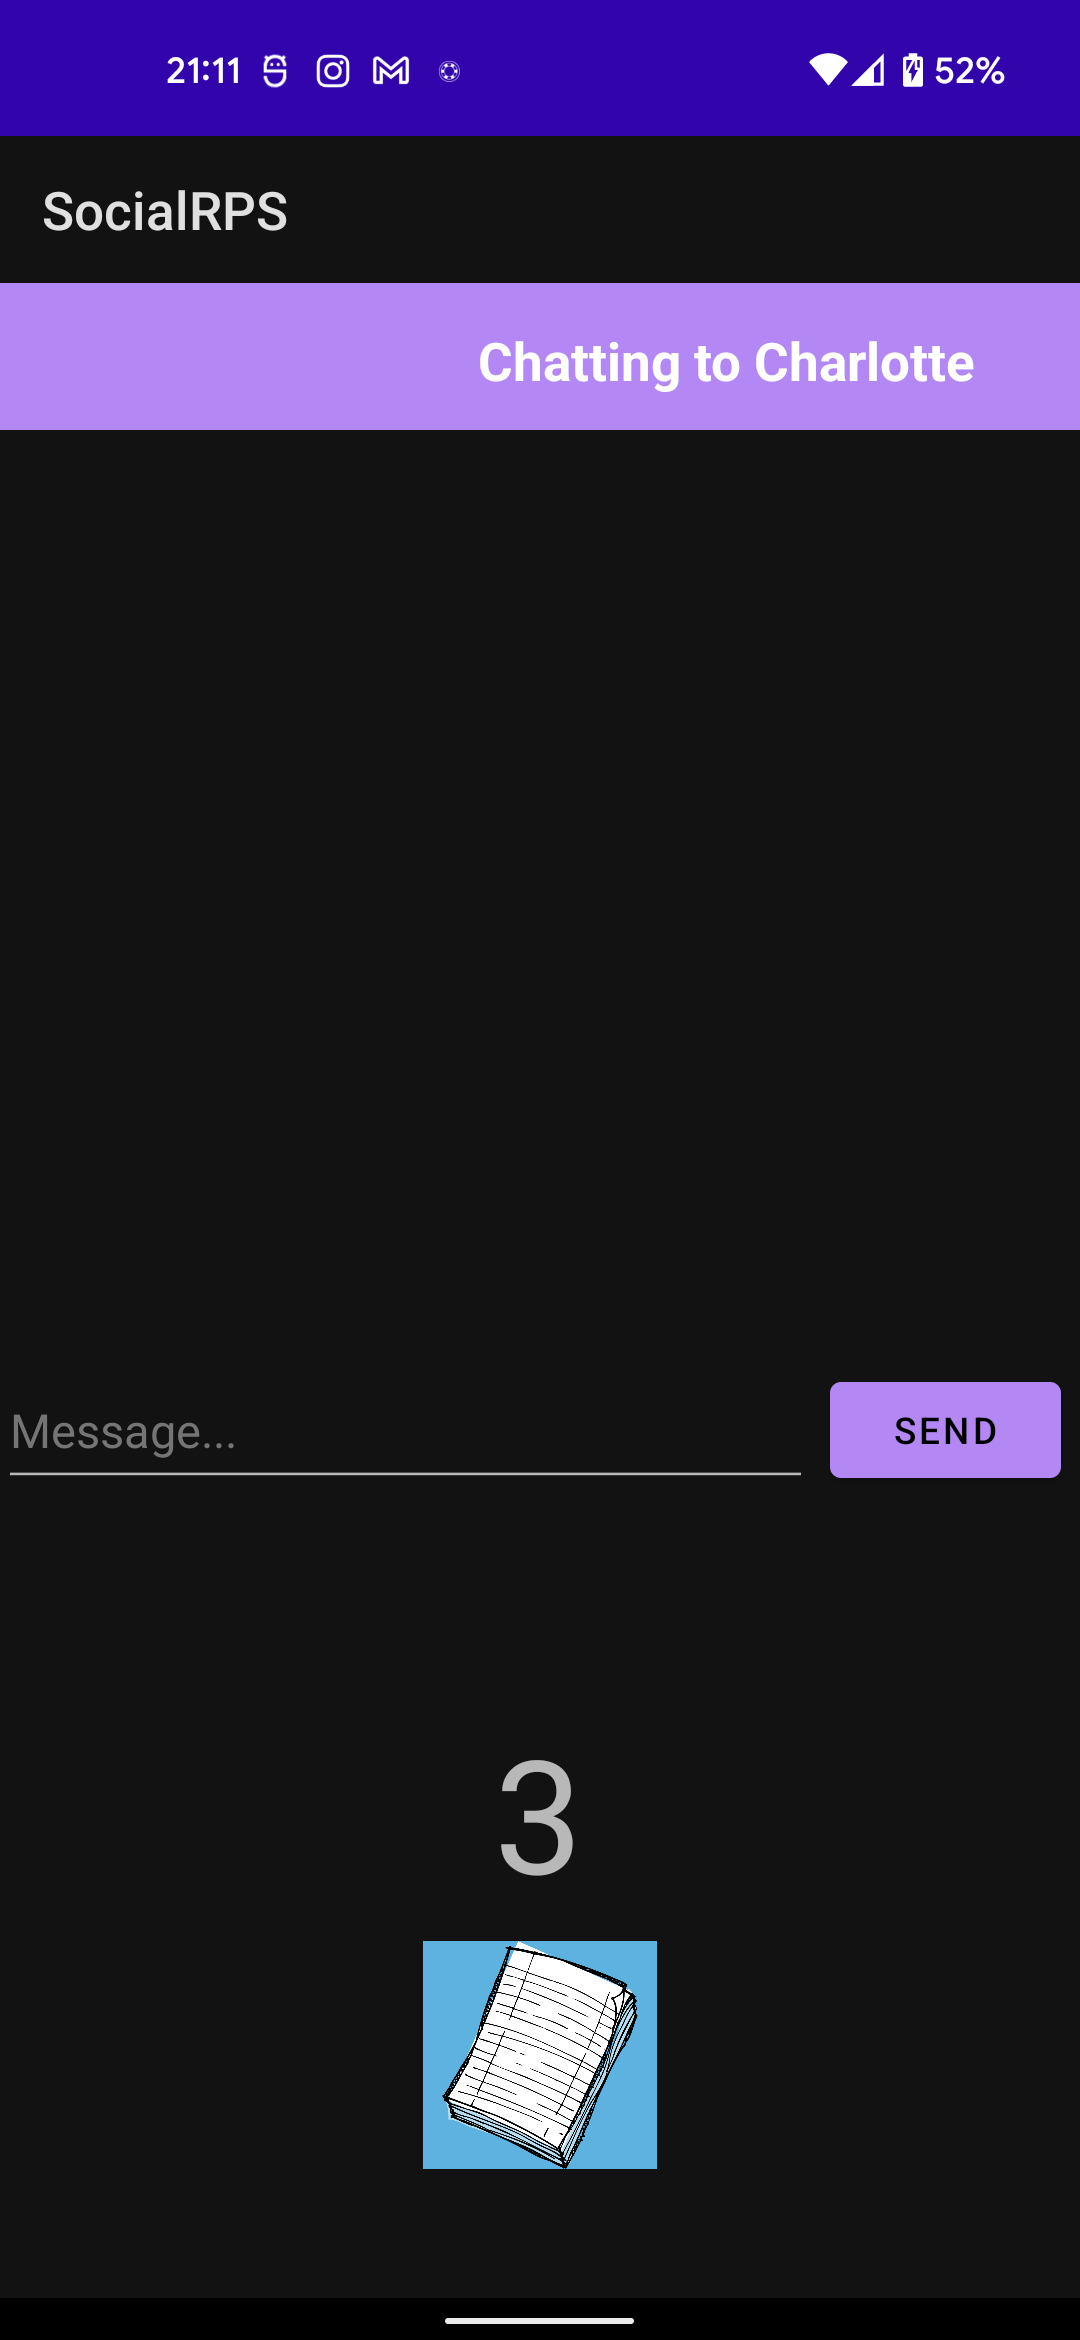
\includegraphics[width=0.27\columnwidth]{Figures/PaperAction.png}
        \caption{Play Game Activity - Paper Action}
        \label{fig:actionsPaper}
      \end{figure}

      Figure~\ref{fig:actionsScissors}: The figure shows what the client sees if the user touches the Scissors action button.
      \begin{figure}[h]
        \centering
        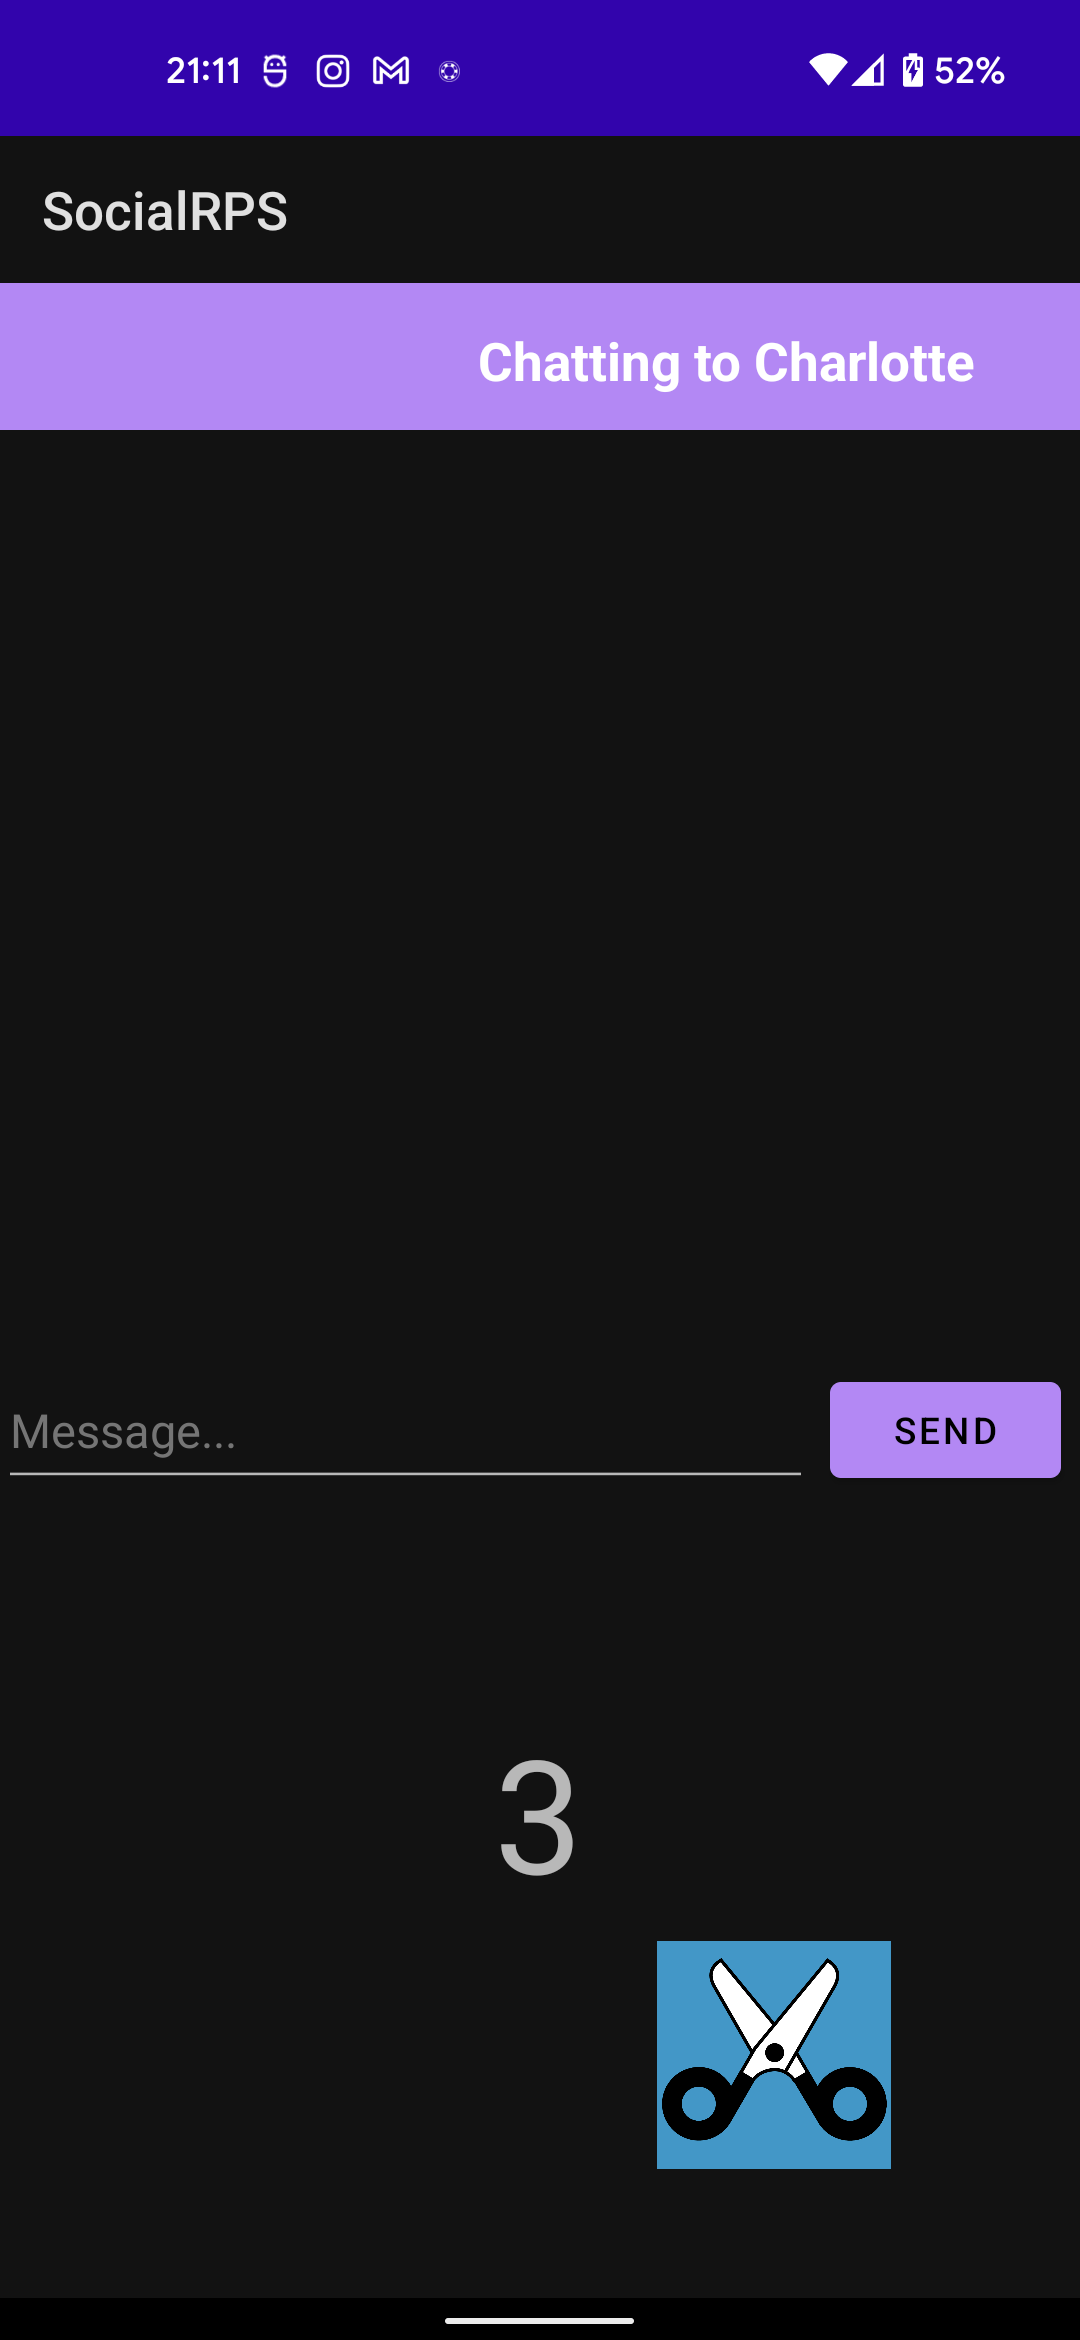
\includegraphics[width=0.27\columnwidth]{Figures/ScissorAction.png}
        \caption{Play Game Activity - Scissors Action}
        \label{fig:actionsScissors}
      \end{figure}

    \section{Conclusion}
    The network protocols provide other communications, whether for data transfer to receiving messages or time synchronisation. The network models help provide insight into how the communication protocols work and help reverse engineer protocols and a template to implement new protocols for future development. After researching the different network protocols' performance, it helps understand how a protocol works and shows the best ways to choose which protocol to use depending on the networking problem.

    \section{Terminology}
      \begin{itemize}
        \item \textbf{TCP:} Transmission Control Protocol.
        \item \textbf{UDP:} User Datagram Protocol.
        \item \textbf{MTU:} Maximum Transmission Unit.
        \item \textbf{OSI:} Open Systems Interconnection.
        \item \textbf{IoT:} Internet of Things.
        \item \textbf{MB:} Megabytes.
        \item \textbf{IP:} Internet Protocol.
        \item \textbf{ICN:} Information-Centric Networks.
        \item \textbf{WWW:} World-Wide Web.
        \item \textbf{NTP:} Network Time Protocol.
        \item \textbf{GNSS:} Global Navigation Satellite System.
        \item \textbf{UTC:} Coordinated Universal Time.
        \item \textbf{GPS:} Global Positioning System.
      \end{itemize}

  \nocite{*}
	\renewcommand\refname{\section{Reference List}}
	\small{\bibliographystyle{IEEEtran}
    \bibliography{ref}}
\end{document}